\chapter{Getting started}
\label{ch:getting-started}

Effective usage of the LISA system requires that you:
\begin{enumerate}
\item{have a basic understanding of how the LISA system is organized;}
\item{know how to copy files from your local machine to LISA and back using SFTP;}
\item{know how to establish an SSH connection, linking your local machine to the LISA system;}
\item{have a basic understanding of the Linux commands that are needed to tell the LISA system what it is you want to do.}
\end{enumerate}



\section{Cluster computing}

A \textit{cluster computer}\index{cluster computer} is a system of interconnected computers that work together so that in many respects they can be viewed as a single system. Clusters usually consist of regular \mbox{off-the-shelf} computers such as those you may find in any computer retail shop (see Fig.~\ref{fig:photo-cluster-computer-uchemnitz}). Cluster computers are especially suited for solving a certain class of computational problems, namely those problems that can be divided into smaller, independently solvable tasks. As a trivial example, finding the minimum value in a 2-D array of values (i.e. a map) is such a problem: the map can be split into two parts and sent to two separate machines. After both machines have found the minimum value in the part of the map that they were assigned, the `global' minimum can be determined by simply comparing the two values. Dividing the task over two or more machines (or actually, \textit{cores}\index{core}) is called \textit{parallelization}\index{parallelization}. Parallelization can greatly reduce the \textit{walltime}\index{walltime} of a computational task (i.e. the time between starting a task and knowing the solution). 

\begin{figure}[htb]
  \centering
    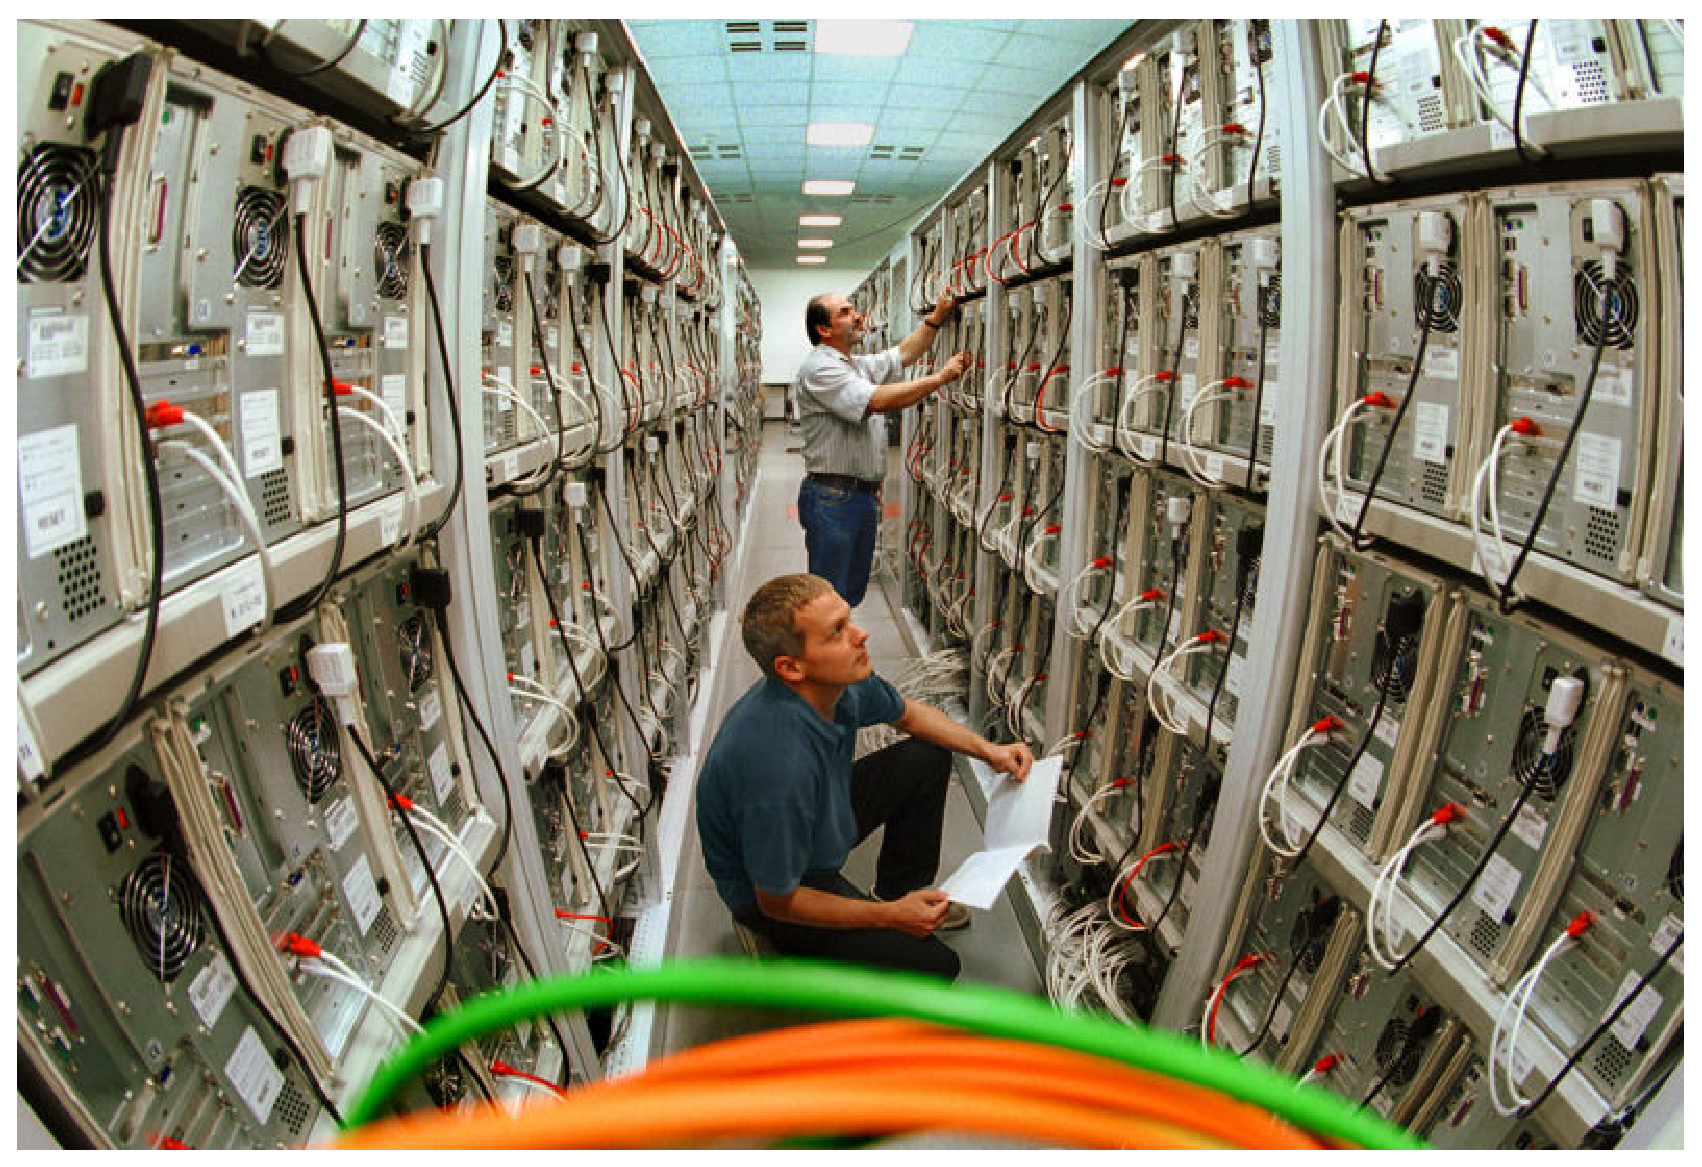
\includegraphics[width=\textwidth]{./../eps/photo-cluster-computer-uchemnitz.eps}
  \caption{Technicians at work on a real cluster computer. Photo from \burl{http://en.wikipedia.org/wiki/File:MEGWARE.CLIC.jpg}.}
  \label{fig:photo-cluster-computer-uchemnitz}
\end{figure}


\section{The LISA cluster: hardware}\index{LISA}

The LISA cluster currently\footnote{LISA's hardware is subject to regular upgrades. For concurrent information, see \burl{https://www.sara.nl/systems/lisa/description\#System_configuration}} consists of 624 normal computers, which are referred to as \textit{nodes}\index{node}. In terms of hardware, each node has a Central Processing Unit (CPU), disk storage, and memory. The nodes are interconnected using a Local Area Network (LAN\index{LAN}). The LAN has low latency and high bandwidth (Gigabit\index{Gigabit} or Infiniband\index{Infiniband}), meaning that in terms of time it is cheap to send large files (because of the high bandwidth) as well as small files (because of the low latency). Storage space on each node varies a little bit, but at the time of writing is 70--220 GB per node. Most nodes have 8-core CPUs, although some have 12-cores or 16-cores. The clock frequency for individual cores is 1.80--2.26 GHz. In terms of memory, most nodes have 24 GB, but the 16-cores have 32 GB. Furthermore, the bandwidth between memory and CPU varies between 5.86--8.00 GT/s. Finally, all nodes run the Debian Linux AMD64 operating system.



\section{Transferring files to and from the LISA cluster}

This section documents the necessary steps for connecting to the LISA cluster from a local Windows machine. First, make sure that you have an account for accessing LISA\footnote{You can get an account by following the instructions from \url{https://www.sara.nl/systems/lisa/account}}. In order to use the cluster effectively, you need to be able to copy files to and from your user directory on the cluster. The LISA cluster is set up such that it exclusively allows connections that are secure, such as Secure File Transfer Protocol (SFTP\index{SFTP}) connections or Secure Shell (SSH\index{SSH}) connections. There are many programs that can establish secure connections, but we will use WinSCP\index{WinSCP}.

Download WinSCP from \burl{http://sourceforge.net/projects/winscp/files/WinSCP/4.3.7/winscp437.zip/download}\footnote{By the time you read this, there may be a more recent version available---just substitute `4.3.7' and `437' from the address with the version you want. For an overview of available versions, look here: \burl{http://sourceforge.net/projects/winscp/files/WinSCP/}.}\footnote{Life is somewhat easier for Linux users. Most Linux distributions come with built-in support for secure connections. Just start up your regular file browser (e.g. PCManFM, Thunar, Nautilus, etc) and type in the address bar \burl{sftp://jspaaks@lisa.sara.nl/home/jspaaks}. Don't forget to substitute your own username. This should automatically establish a connection between your machine and the remote system (i.e. the cluster). Fill in your credentials when prompted.}. Unzip into your home directory or a USB drive. Double-click on `WinSCP.exe' to start the WinSCP program. The program will prompt you for some input (see Fig.~\ref{fig:winscp-session-dialog}). Under `Host name:', fill in `lisa.sara.nl'. Make sure that the port number is set to `22'. Under `User name:', fill in your LISA cluster username. You can leave the `Password' field blank, the program will prompt you later. Make sure `SFTP' is selected as the file protocol. Click on `Save...' to store these settings if you like. Then press the `Login' button to establish the SFTP connection to the LISA cluster. The program will throw a warning about the RSA key fingerprint file. The number shown in the warning dialog should be the same as the number posted at \burl{https://www.sara.nl/systems/shared/ssh} (table at the bottom of the web page). If it is, press `Yes' and then `Continue' in the next dialog box. As a final step, fill in your password when prompted. You should now see two panes, one for the local machine on the left and one for the remote machine, i.e. the LISA cluster, on the right (see Fig.~\ref{fig:winscp-two-panes}).

\begin{figure}[htbp]
  \centering
    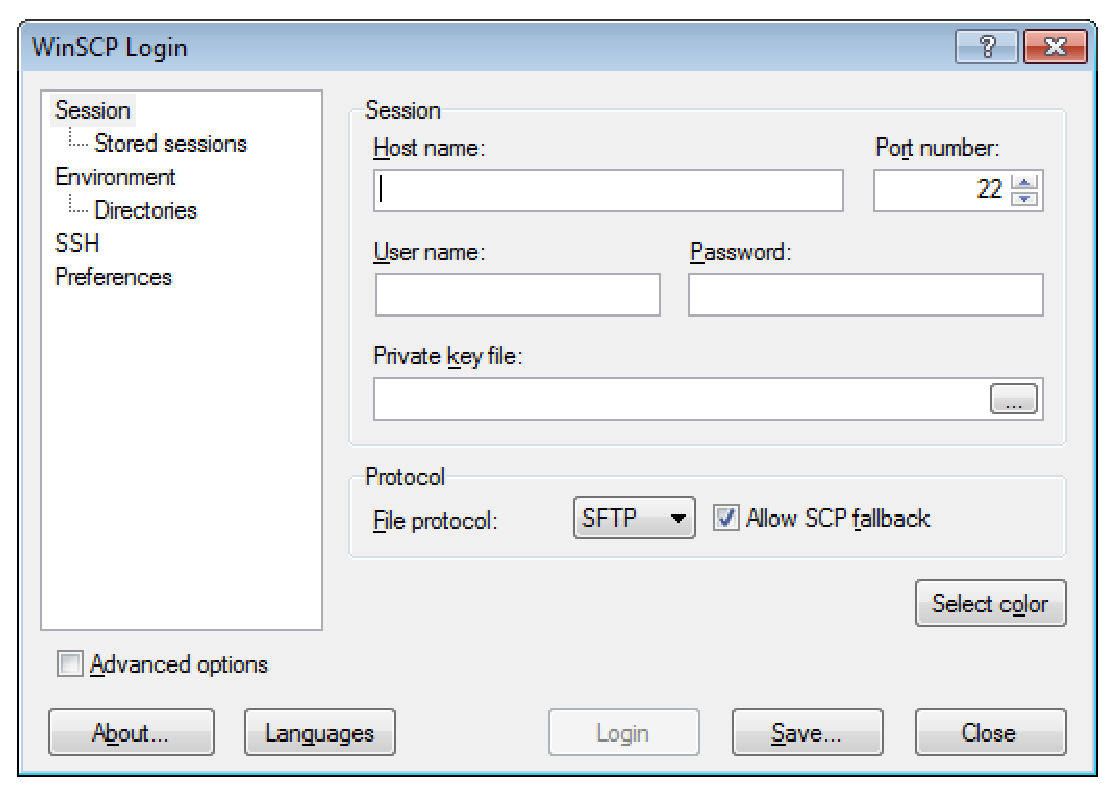
\includegraphics[width=0.5\textwidth]{./../eps/winscp-session-dialog.eps}
  \caption{WinSCP session dialog box.}
  \label{fig:winscp-session-dialog}
\end{figure}

\begin{figure}[htbp]
  \centering
    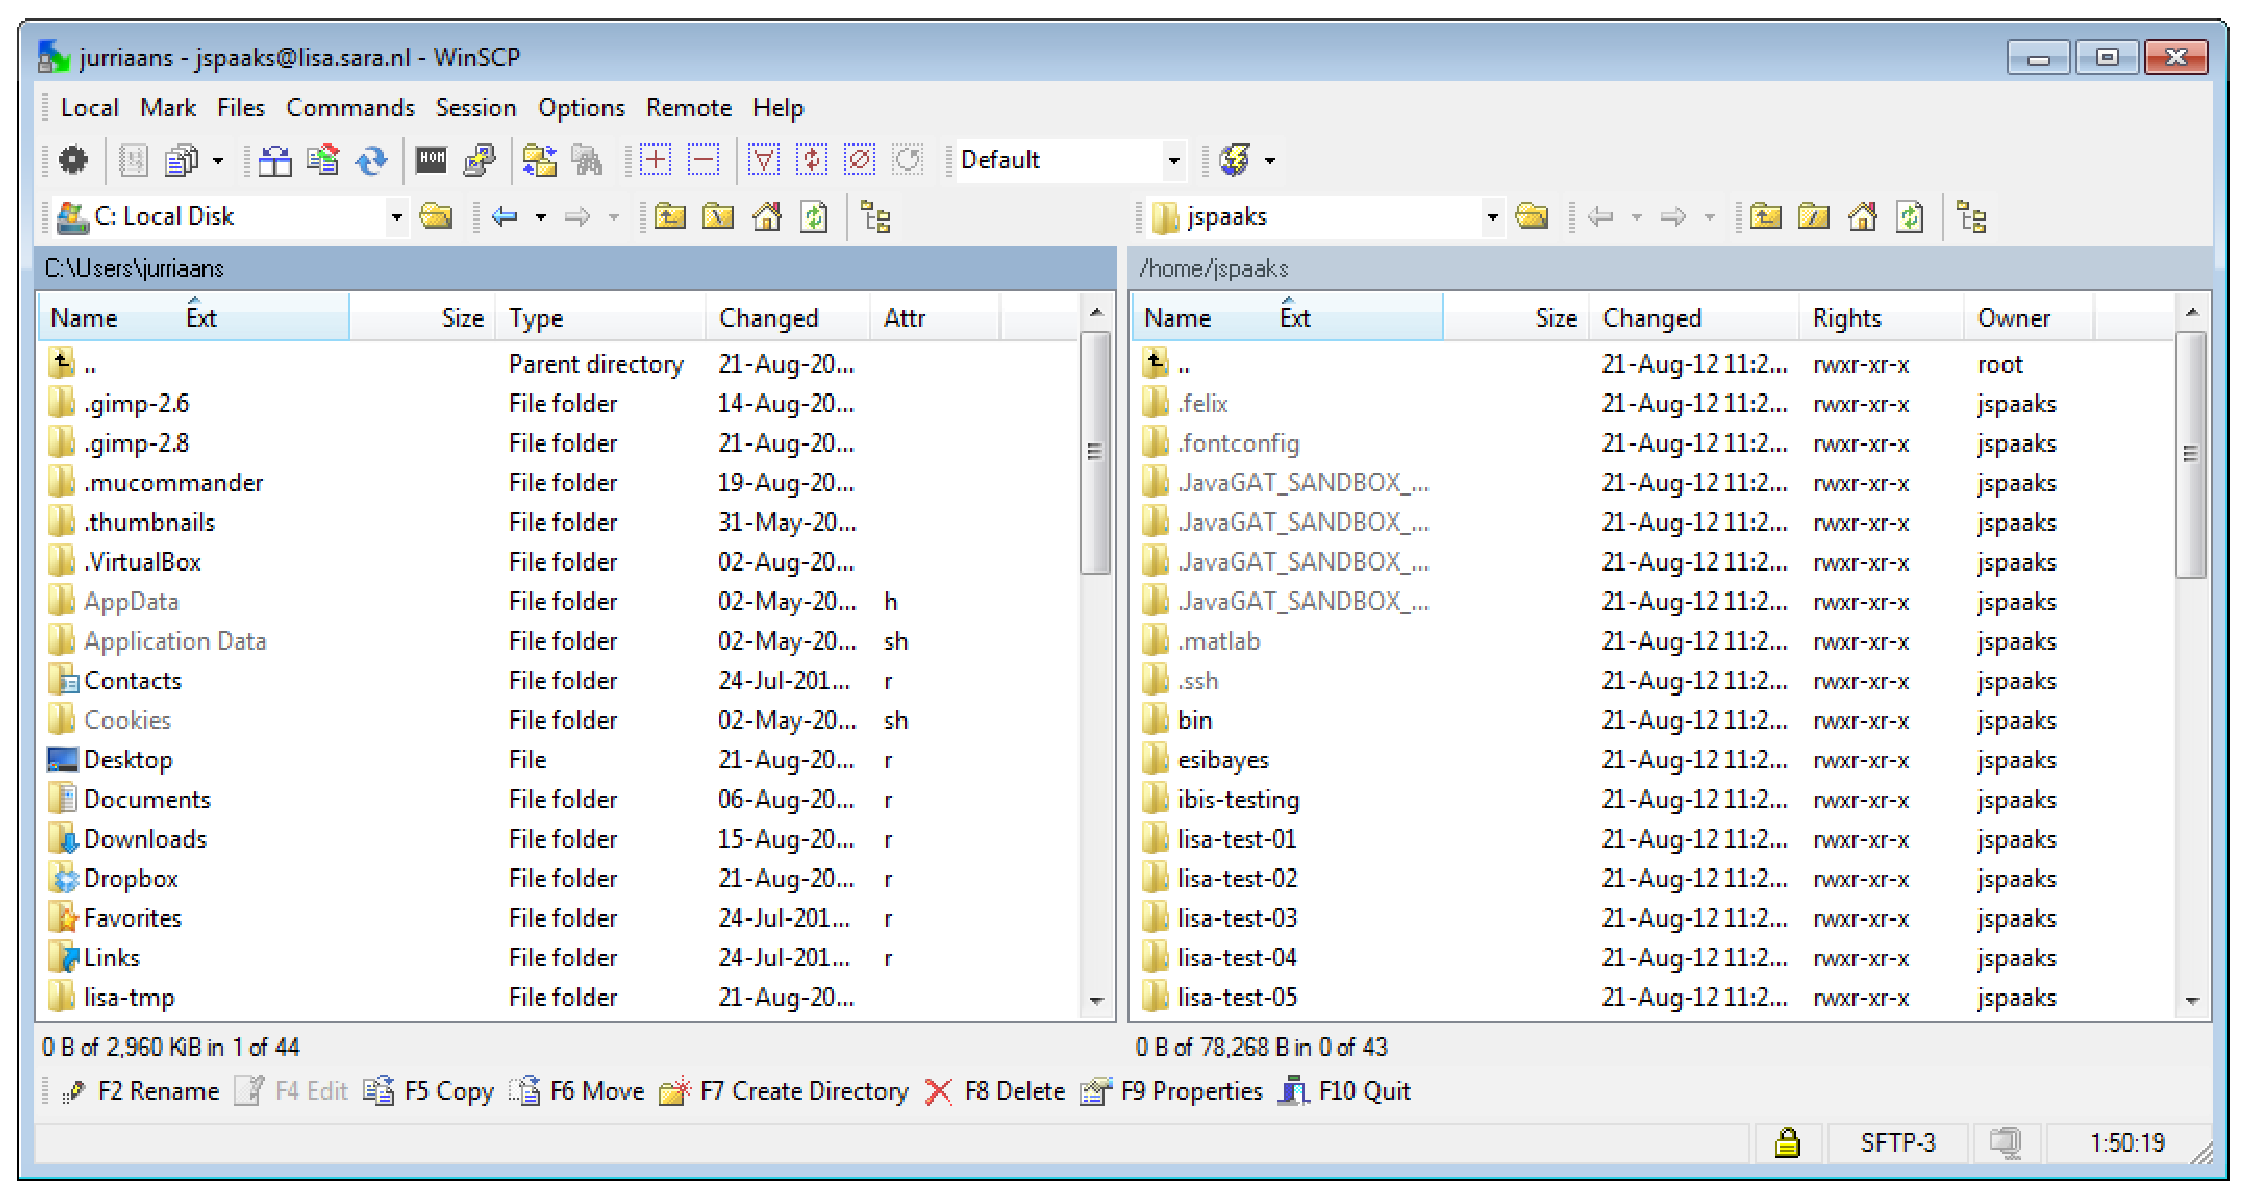
\includegraphics[width=1.0\textwidth]{./../eps/winscp-two-panes.eps}
  \caption{WinSCP interface. On the left is my local file system, on the right is my home directory on the remote file system. If this is the first time you connect to LISA, the remote file system should be pretty much empty.}
  \label{fig:winscp-two-panes}
\end{figure}

Download `tutorial.zip' from \url{http:\\www.????.??} and unzip into your (local) home directory or a USB drive.

In WinSCP, use the left pane to navigate to the directory where you unzipped the tutorial files. Copy the `tutorial' folder to the remote directory by selecting it on the left and pressing the F5 button. The tutorial folder should now be present in the right pane as well.


\section{Issuing commands on the LISA cluster}
This section covers how you can issue commands from your local machine, which then get executed by the remote system (LISA). Issuing commands on the LISA cluster can be accomplished through a so-called terminal emulator program\index{terminal emulator}. A terminal emulator provides you with a prompt at which you can type commands which are then executed on the remote system. It doesn't matter whether the remote system is located just across the street or halfway around the world, you can still operate it through the terminal emulator. However, it is important to note that the LISA cluster, like virtually all clusters\footnote{See \burl{http://i.top500.org/stats} for concurrent statistics on the World's top 500 of supercomputers.}, runs under the Linux operating system. The commands that you type at the terminal emulator prompt therefore need to be Linux commands, which, as you will see later, are somewhat different from the Windows commands that you may be familiar with.

%
Let's first download the terminal emulator PuTTY\index{PuTTY} from \url{http://www.chiark.greenend.org.uk/~sgtatham/putty/download.html} into your home directory. Double-click the executable to run the program. You should now see the dialog from Fig.~\ref{fig:putty-session-dialog}. Under `Host name or IP address', fill in `lisa.sara.nl' and press the `Open' button. PuTTY first prompts you for your username and then for your password. Fill in your LISA credentials.\footnote{On Linux, bring up a terminal (Ctrl-Alt-t on most distributions) and type in \texttt{ssh jspaaks@lisa.sara.nl}, substituing your own username in stead of \texttt{jspaaks}. Fill in your credentials when prompted.}

\begin{figure}[htbp]
  \centering
    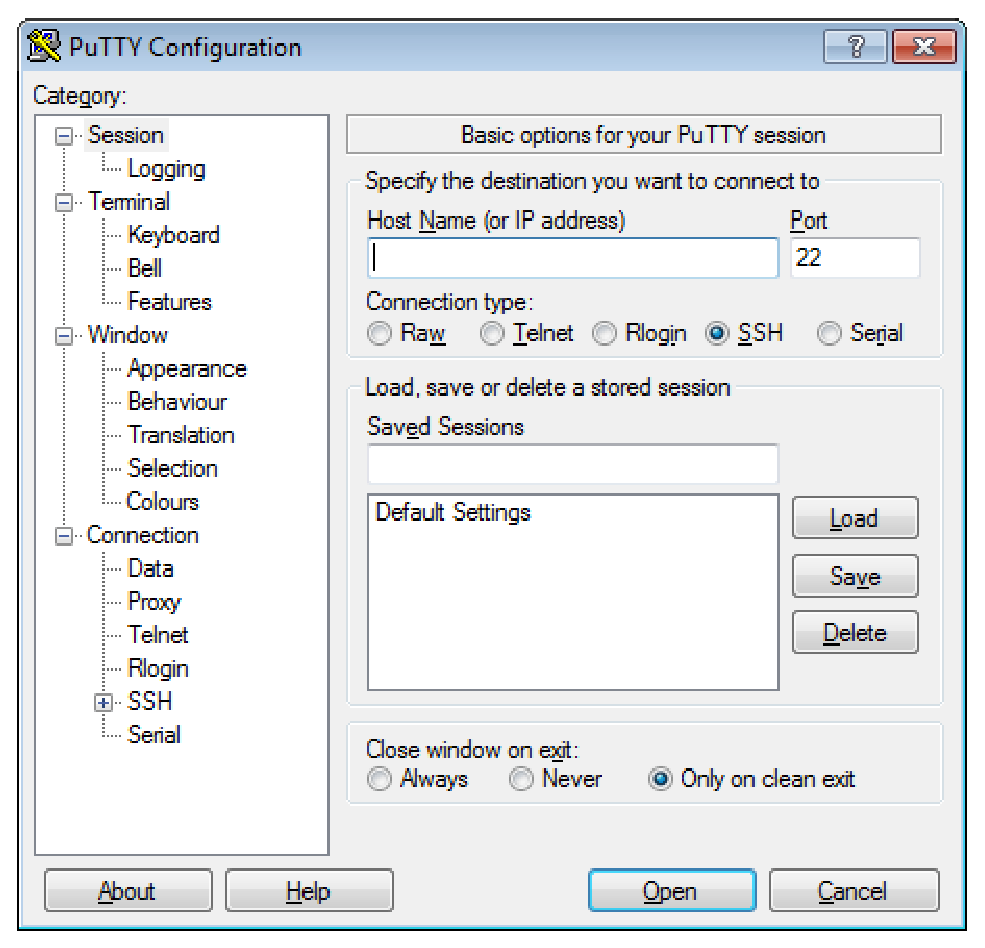
\includegraphics[width=0.5\textwidth]{./../eps/putty-session-dialog.eps}
  \caption{PuTTY session dialog box.}
  \label{fig:putty-session-dialog}
\end{figure}


You are now remotely logged in to the Linux cluster LISA. Your terminal emulator program should show something like:
\begin{lstlisting}[style=basic,style=bash]
jspaaks@login4:~$
\end{lstlisting}
where \texttt{jspaaks} is the username and \texttt{login4}\index{login4@\texttt{login4}} is the name of the remote machine. There are, in fact, two machines on which you can log in remotely: besides \lstinline[style=bashinline]{login4}, there's also \lstinline[style=bashinline]{login3}\index{login3@\texttt{login3}}. For our intents and purposes, it doesn't matter whether you are logged in to \lstinline[style=bashinline]{login3} or \lstinline[style=bashinline]{login4}, but if you want to change from one to the other, you can do so with:
\begin{lstlisting}[style=basic,style=bash]
jspaaks@login4:~$ ssh login3
\end{lstlisting}

When you're done with the terminal, you can close the connection using: 
\index{Linux commands!logout@\texttt{logout}}
\begin{lstlisting}[style=basic,style=bash]
jspaaks@login4:~$ logout
\end{lstlisting}


If you want to find out in which directory you are, you can use the \lstinline[style=bashinline]{pwd}\index{Linux commands!pwd@\texttt{pwd}} command (`pwd' is short for present working directory):
\begin{lstlisting}[style=basic,style=bash]
jspaaks@login4:~$ pwd
\end{lstlisting}
which returns:
\begin{lstlisting}[style=basic,style=bash]
/home/jspaaks
\end{lstlisting}
It is worth noting that a list of useful commands and terms has been included in the Index section at the back of this document.

So, \texttt{pwd} returns \texttt{/home/jspaaks/}. \texttt{/home/jspaaks/} is the user's home directory; it is the Linux equivalent of `C:\textbackslash{}Users\textbackslash{}jspaaks' on Windows. Note that on Linux the directory separator \index{/@\texttt{/} (directory separator, Linux)} is the forward slash `/' sign, whereas~Windows uses the backslash `\textbackslash{}'\index{\textbackslash{}@\texttt{\char`\\
} (directory separator, Windows)} sign. You may be wondering why there isn't a `C:\textbackslash{}' in the address returned by \texttt{pwd}. The reason is simple: Linux uses `/'\index{/@\texttt{/} (file system root, Linux)}\index{root@root (file system)} instead of `C:\textbackslash{}' \footnote{Somewhat confusingly, the account that has Administrator privileges is also referred to as `root' on Linux systems.\index{root@root (system administrator)}}. The first forward slash in the address is referred to as the `file system root'. Under the file system root is a directory `home', which contains a subdirectory `jspaaks' in which the user `jspaaks' keeps all his personal files. As a matter of fact, \texttt{/home/jspaaks} is the only place on this file system that user `jspaaks' is permitted to write anything, meaning that Linux will not allow you to save any files in other users' home directories (although you are allowed to read some of them, depending on how the \textit{permissions}\index{permission} on that directory are set. More about permissions later).

You can view the contents of the current directory using the \texttt{ls} (short for `list') command:\index{Linux commands!ls@\texttt{ls}}
\begin{lstlisting}[style=basic,style=bash]
jspaaks@login4:~$ ls
\end{lstlisting}
This should show at least the `tutorial' folder that we just copied using WinSCP.

Changing the current working directory works in a similar way as at the Command Prompt on Windows:
\begin{lstlisting}[style=basic,style=bash]
jspaaks@login4:~$ cd tutorial
jspaaks@login4:~/tutorial$ 
\end{lstlisting}\index{Linux commands!cd@\texttt{cd}}
Note that the prompt includes the location of the current directory: `\textasciitilde' (pronounced: `tilde') represents the home directory (`/home/jspaaks').
Changing to the current working directory from any location on the file system to the user's home directory goes like so:
\begin{lstlisting}[style=basic,style=bash]
jspaaks@login4:~/tutorial/a/really/deeply/nested/directory$ cd ~
jspaaks@login4:~$ 
\end{lstlisting}
or if you want to move just one directory up:
\begin{lstlisting}[style=basic,style=bash]
jspaaks@login4:~/tutorial/a/really/deeply/nested/directory$ cd ..
jspaaks@login4:~/tutorial/a/really/deeply/nested$ 
\end{lstlisting}
make sure to include the space character in between the \texttt{cd} and \texttt{..} characters though, otherwise it won't work.

A new directory can be created by the \texttt{mkdir}\index{Linux commands!mkdir@\texttt{mkdir}} command, for example:
\begin{lstlisting}[style=basic,style=bash]
jspaaks@login4:~$ mkdir anewdir
\end{lstlisting}\index{Linux commands!mkdir@\texttt{mkdir}}
Note that, contrary to Windows file systems, Linux file systems are case-sensitive. For example:
\begin{lstlisting}[style=basic,style=bash]
jspaaks@login4:~$ mkdir aNewDir
\end{lstlisting}
will result in an additional directory:
\begin{lstlisting}[style=basic,style=bash]
jspaaks@login4:~$ ls
anewdir   aNewDir   tutorial
jspaaks@login4:~$ 
\end{lstlisting}
The different approaches that Windows and Linux take in regard to case-sensitivity of their respective file systems can lead to errors, especially when copying back and forth between Windows and Linux systems. For example, the contents of \lstinline{anewdir} and \lstinline{aNewDir} may get merged when they are copied to a Windows system, since Windows regards the folders as being one and the same. To avoid these kinds of errors, the naming convention on Linux is to use only lower caps names for files and folders, so \lstinline{anewdir} is preferable to  \lstinline{aNewDir}. 

Regardless of your native operating system, your code will be more robust and more portable if you stick to these 2~simple rules when naming your files:
\begin{enumerate}
\item{don't use spaces;}
\item{limit yourself to the following subset of characters:\\ \lstinline[style=bashinline]{abcdefghijklmnopqrstuvwxyz_-.0123456789},\\ and, if you must, \lstinline[style=bashinline]{ABCDEFGHIJKLMNOPQRSTUVWXYZ} .}\footnote{You'll thank me later!}
\end{enumerate}



Removing a directory goes like this:
\begin{lstlisting}[style=basic,style=bash]
jspaaks@login4:~$ rmdir aNewDir
\end{lstlisting}\index{Linux commands!rmdir@\texttt{rmdir}}
or like this if you want to remove multiple directories:
\begin{lstlisting}[style=basic,style=bash]
jspaaks@login4:~$ rmdir anewdir aNewDir 
\end{lstlisting}


For many commands, you can specify options. Options to a given command must generally be provided directly after the command itself, i.e.~before any other argument such as input or output files.  The option argument consists of one dash followed by one (case-sensitive) letter. For example, if you want \texttt{ls} to list the contents of the current directory in more detail, you can use the \texttt{-l} option (that is the letter~\textit{l} for `long', not the number~1):
\begin{lstlisting}[style=basic,style=bash]
jspaaks@login4:~$ ls -l
total 4
drwxrwxr-x 2 jspaaks jspaaks 2 Jun 13 13:07 tutorial
\end{lstlisting}
which gives you, amongst other things, the \textit{permission bits}\index{permission bits} (i.e.\,\lstinline{drwxrwxr-x}), the owner of the item (\lstinline{jspaaks}), the item's size (\lstinline{2}) in bytes and the time when the item was last altered (\lstinline{Jun 13 13:07}). Note that, by default, \lstinline[style=bashinline]{ls} sorts the items in a directory based on the item's name, so directories and files will appear intermingled. You can easily tell whether an item is one or the other by looking at the permission bits: if the item is a folder, the first character that appears in the permission bits is the letter \lstinline[style=bashinline]{d}. For files, the first character in the permission bits is \lstinline[style=bashinline]{-}.

Most Linux commands have at least a few optional arguments. If you want to know more about a particular command's usage, you can use the \texttt{man}\index{Linux commands!man@\texttt{man}} (short for `manual') command, which lists all the options for a given program including a short description of what each option does. For example, try:
\begin{lstlisting}[style=basic,style=bash]
jspaaks@login4:~$ man ls
\end{lstlisting}
(you can scroll down using the `Up' and `Down' arrows. Pressing the `q' key lets you return to the prompt). If you just want to verify that you remember the command right, you can check by: 
\begin{lstlisting}[style=basic,style=bash]
jspaaks@login4:~$ whatis ls
ls (1)               - list directory contents
\end{lstlisting}
which will give you a short summary of what \lstinline{ls} is doing, but without all the technical detail.

In addition to the shorthand notation, some options also have a longer version for improved readibility. The longer version always starts with two dashes instead of one. As an example, the \lstinline[style=bashinline]{-h} option makes \lstinline[style=bashinline]{ls} list the filesizes in more easily interpretable units such as kB or MB, rather than in bytes:
\begin{lstlisting}[style=basic,style=bash]
jspaaks@login4:~$ ls -l -h
\end{lstlisting}
or, combining the shorthand options:
\begin{lstlisting}[style=basic,style=bash]
jspaaks@login4:~$ ls -lh
\end{lstlisting}
The longer version of the \lstinline[style=bashinline]{-h} option is \lstinline[style=bashinline]{--human-readable}, so the complete command becomes: 
\begin{lstlisting}[style=basic,style=bash]
jspaaks@login4:~$ ls -l --human-readable
\end{lstlisting}


Now that you know a little bit about Linux, let's look at how to manipulate files. \lstinline[style=bashinline]{cd} into the `deeply nested directory' by typing:
\begin{lstlisting}[style=basic,style=bash]
jspaaks@login4:~$ cd tu
\end{lstlisting}
if you now press Tab, the \textit{shell}\index{shell} program (i.e.\,the program that lets you enter commands at the prompt) will automatically complete your command, like so:\index{Linux commands!autocompletion}
\begin{lstlisting}[style=basic,style=bash]
jspaaks@login4:~$ cd tutorial
\end{lstlisting}
This autocomplete works because the shell knows that you want to do a \lstinline[style=bashinline]{cd}, and since there is only one directory in \textasciitilde{} that starts with \lstinline[style=bashinline]{tu}, the shell program knows that you want to \lstinline[style=bashinline]{cd} into \lstinline[style=bashinline]{tutorial}.

If you \lstinline[style=bashinline]{cd} into \lstinline{a/really/deeply/nested/directory} and list the directory contents, there should be a file called `with-a-file-in-it.txt'. Because this is an \mbox{ASCII} text file, you can display it in the shell program by using the command \lstinline[style=bashinline]{cat}\index{Linux commands!cat@\texttt{cat}}, like so:
\begin{lstlisting}[style=basic,style=bash]
jspaaks@login4:~/tutorial/a/really/deeply/nested/directory$ cat with-a-file-in-it.txt
\end{lstlisting}

\lstinline[style=bashinline]{cat} is short for `concatentate', meaning it appends the contents of `with-a-file-in-it.txt' to whatever is already displayed within the shell. Also note that autocomplete works here as well, but instead of listing any directory names, it will suggest a file from the current directory, since that is the kind of argument that \lstinline[style=bashinline]{cat} expects. You will see the following output:
\begin{lstlisting}[style=basic,style=bash]
jspaaks@login4:~$ cd tutorial/a/really/deeply/nested/directory/
jspaaks@login4:~/tutorial/a/really/deeply/nested/directory$ ls
with-a-file-in-it.txt
jspaaks@login4:~/tutorial/a/really/deeply/nested/directory$ cat with-a-file-in-it.txt 
* * * * * * * * * * * * * * * * * * * * *
* *                                   * *
* *  hello world, the classic phrase  * *
* *                                   * *
* * * * * * * * * * * * * * * * * * * * *
jspaaks@login4:~/tutorial/a/really/deeply/nested/directory$ 
\end{lstlisting}
(the lines that start with asterisks are actually the contents of `with-a-file-in-it.txt'.)

Let's now try to move this file to the top directory in the user's home by using the move command \lstinline[style=bashinline]{mv}\index{Linux commands!mv@\texttt{mv}}\index{Linux commands!move} like so:
\begin{lstlisting}[style=basic,style=bash]
jspaaks@login4:~/tutorial/a/really/deeply/nested/directory$ mv with-a-file-in-it.txt ~
\end{lstlisting}
The syntax for this command is the command itself, i.e.~\lstinline[style=bashinline]{mv}, followed by a space, followed by the first input argument, in this case the name of the file that we want to move, i.e.~\lstinline[style=bashinline]{with-a-file-in-it.txt}, followed by another space, followed by the name of the directory that we want to move it to \lstinline[style=bashinline]{~}. Also note that autocomplete works here as well, just type \lstinline[style=bashinline]{mv wit} and press Tab to autocomplete.

Let's check that the file really got moved:
\begin{lstlisting}[style=basic,style=bash]
jspaaks@login4:~/tutorial/a/really/deeply/nested/directory$ cd ~
jspaaks@login4:~$ ls -l
total 6
drwxr-xr-x  4 jspaaks jspaaks    4 Aug 20 11:59 tutorial
-rw-r--r--  1 jspaaks jspaaks  210 Aug 20 15:21 with-a-file-in-it.txt
jspaaks@login4:~$  
\end{lstlisting}

You can also use the \lstinline[style=bashinline]{mv} command to rename\index{Linux commands!rename} a file by `moving' it to a different filename in the same directory like so:
\begin{lstlisting}[style=basic,style=bash]
jspaaks@login4:~$ ls -l
total 6
drwxr-xr-x  5 jspaaks jspaaks    5 Aug 21 14:45 tutorial
-rw-r--r--  1 jspaaks jspaaks  210 Aug 20 15:21 with-a-file-in-it.txt
jspaaks@login4:~$ mv with-a-file-in-it.txt the-renamed-file.txt 
jspaaks@login4:~$ ls -l
total 6
-rw-r--r--  1 jspaaks jspaaks  210 Aug 20 15:21 the-renamed-file.txt
drwxr-xr-x  5 jspaaks jspaaks    5 Aug 21 14:45 tutorial
jspaaks@login4:~$ 
\end{lstlisting}


Now suppose we don't want to move a file but we want to copy it. This can be done using the \lstinline[style=bashinline]{cp}\index{Linux commands!cp@\texttt{cp}}\index{Linux commands!copy} command. For example:
\begin{lstlisting}[style=basic,style=bash]
jspaaks@login4:~$ cp with-a-file-in-it.txt copy-of-the-text-file 
\end{lstlisting}
The copy command \lstinline[style=bashinline]{cp} expects the file-to-be-copied as its first argument, and the name of the file-to-copy-to as its second argument. Further note that you don't have to specify extensions such as `.txt' in the filename for the operating system to know that \lstinline[style=bashinline]{copy-of-the-text-file} is a text file, as you would normally do on Windows. Nevertheless, including the extension in the file name allows easy identification of the type of file, for example when listing the contents of a directory with \lstinline[style=bashinline]{ls}, especially when combined with wildcards such as \lstinline[style=bashinline]{*}:

\begin{lstlisting}[style=basic,style=bash]
jspaaks@login4:~/tutorial/a$ ls -l
total 10
-rw-rw-r-- 1 jspaaks jspaaks 16 Aug 22 10:02 file1.txt
-rw-rw-r-- 1 jspaaks jspaaks 16 Aug 22 10:00 file2.txt
-rw-rw-r-- 1 jspaaks jspaaks 16 Aug 22 10:00 file3.txt
-rw-rw-r-- 1 jspaaks jspaaks 13 Aug 22 10:02 file4.m
-rw-rw-r-- 1 jspaaks jspaaks 13 Aug 22 10:01 file5.m
drwxr-xr-x 3 jspaaks jspaaks  3 Aug 20 11:56 really
jspaaks@login4:~/tutorial/a$ ls -l *.txt
-rw-rw-r-- 1 jspaaks jspaaks 16 Aug 22 10:02 file1.txt
-rw-rw-r-- 1 jspaaks jspaaks 16 Aug 22 10:00 file2.txt
-rw-rw-r-- 1 jspaaks jspaaks 16 Aug 22 10:00 file3.txt
jspaaks@login4:~/tutorial/a$ 
\end{lstlisting}


\lstinline{cp} also lets you copy directories, like so:
\begin{lstlisting}[style=basic,style=bash,style=numbered]
jspaaks@login4:~$ cd tutorial
jspaaks@login4:~/tutorial$ ls -l
total 5
drwxr-xr-x 3 jspaaks jspaaks 3 Aug 20 11:56 a
drwxr-xr-x 2 jspaaks jspaaks 5 Aug 20 12:07 simple-jobscript
jspaaks@login4:~/tutorial$ mkdir another
jspaaks@login4:~/tutorial$ cp -R a/* another
jspaaks@login4:~/tutorial$ ls -l
total 8
drwxr-xr-x 3 jspaaks jspaaks 3 Aug 20 11:56 a
drwxrwxr-x 3 jspaaks jspaaks 3 Aug 21 14:46 another
drwxr-xr-x 2 jspaaks jspaaks 5 Aug 20 12:07 simple-jobscript
jspaaks@login4:~/tutorial$ cd another/really/deeply/nested/directory/
jspaaks@login4:~/tutorial/another/really/deeply/nested/directory$
\end{lstlisting}
Line 1 changes the current directory to \lstinline[style=bashinline]{tutorial}, line 2 lists its contents, line 6 creates the directory called `another'. The actual copying is subsequently done in line 7. The complete command consists of the \lstinline[style=bashinline]{cp} command, followed by the \lstinline[style=bashinline]{-R} option that makes \lstinline[style=bashinline]{cp} copy recursively, followed by the source files and folders \lstinline[style=bashinline]{a/*} (i.e.~everything under \lstinline[style=bashinline]{~/tutorial/a}), followed by the destination directory \lstinline[style=bashinline]{another}. Line 8 shows the newly created directory, while lines 13--14 show that the copy operation was indeed recursive.

Besides manipulating files and folders, the shell can do a lot more. For example, you can temporarily turn the shell program into a Octave\index{Octave} command window, like so:
\begin{lstlisting}[style=basic,style=bash]
jspaaks@login4:~$ octave
\end{lstlisting}
\index{Linux commands!octave@\texttt{octave}}

The Octave program welcomes you with its default welcome message, followed by a prompt:
\begin{lstlisting}[style=basic,style=bash]
GNU Octave, version 3.2.4
Copyright (C) 2009 John W. Eaton and others.
This is free software; see the source code for copying conditions.
There is ABSOLUTELY NO WARRANTY; not even for MERCHANTABILITY or
FITNESS FOR A PARTICULAR PURPOSE.  For details, type `warranty'.

Octave was configured for "x86_64-pc-linux-gnu".

Additional information about Octave is available at http://www.octave.org.

Please contribute if you find this software useful.
For more information, visit http://www.octave.org/help-wanted.html

Report bugs to <bug@octave.org> (but first, please read
http://www.octave.org/bugs.html to learn how to write a helpful report).

For information about changes from previous versions, type `news'.

octave:1> 
\end{lstlisting}
At the prompt, you can type any Octave command. For example: 
\begin{lstlisting}[style=basic,style=bash]
octave:1> for k=1:4, disp(['The value of ''k'' = ',num2str(k)]),end
The value of 'k' = 1
The value of 'k' = 2
The value of 'k' = 3
The value of 'k' = 4
octave:2> 
\end{lstlisting}
If you want to return to the normal shell, just type: 
\begin{lstlisting}[style=basic,style=bash]
octave:2> exit
\end{lstlisting}

From the example above, you can see that typing everything on the command line can be tricky, even for simple tasks. Wouldn't it be great to have an editor of some kind? You've guessed it, the shell can also be turned into a (very) basic editor, like so:
\begin{lstlisting}[style=basic,style=bash]
jspaaks@login4:~$ nano
\end{lstlisting}
\index{Linux commands!nano@\texttt{nano}}

You can use the nano program to write a simple Octave script, for example the one in Listing~\ref{list:nano-simple-script}:
\begin{lstlisting}[style=numbered,style=basic,style=bash,style=numbered,caption={Example of a simple Octave script in nano.},label=list:nano-simple-script]
  GNU nano 2.2.4                 New Buffer                                   Modified  

% This is a simple octave script example written in Nano

% clear any old variables
clear

for k=1:5
    str = ['The value of ''k'' is ',num2str(k)];
    disp(str)
end





^G Get Help    ^O WriteOut    ^R Read File   ^Y Prev Page   ^K Cut Text    ^C Cur Pos
^X Exit        ^J Justify     ^W Where Is    ^V Next Page   ^U UnCut Text  ^T To Spell
\end{lstlisting}
The first line of Listing~\ref{list:nano-simple-script} consists of the name and version of the nano program, followed by either the filename (if you opened an existing file) or the string \lstinline[style=bashinline]{New Buffer} (if the file has not been saved yet). The string \lstinline[style=bashinline]{Modified} is displayed at the right if the user has made any changes. The bottom two lines list a number of keyboard combinations, where the caret symbol~\lstinline[style=bashinline]{^} represents the Ctrl key, so \lstinline[style=bashinline]{^G} means Ctrl-g. After you've typed your script, you can save it by pressing Ctrl-o, typing the filename that you want your script to have, and pressing Enter. You can exit nano by pressing Ctrl-x. If you happen to press Ctrl-x when your script has not been saved yet, nano will ask you if you want to save it before exiting.

Let's check that the script from Listing~\ref{list:nano-simple-script} was written to file:
\begin{lstlisting}[style=basic,style=bash]
jspaaks@login4:~$ cat simple_octave_script.m 
% This is a simple octave script example written in Nano

% clear any old variables
clear

for k=1:5
    str = ['The value of ''k'' is ',num2str(k)];
    disp(str)
end
jspaaks@login4:~$ 
\end{lstlisting}

Now we can call the Octave program using the name of the script as an input argument like so:
\begin{lstlisting}[style=basic,style=bash]
jspaaks@login4:~$ octave simple_octave_script.m 
\end{lstlisting}
This starts the Octave program, runs the script within it as if you had typed `simple\_octave\_script' at the Octave prompt, and returns to the shell:
\begin{lstlisting}[style=basic,style=bash]
jspaaks@login4:~$ octave simple_octave_script.m 
GNU Octave, version 3.2.4
Copyright (C) 2009 John W. Eaton and others.
This is free software; see the source code for copying conditions.
There is ABSOLUTELY NO WARRANTY; not even for MERCHANTABILITY or
FITNESS FOR A PARTICULAR PURPOSE.  For details, type `warranty'.

Octave was configured for "x86_64-pc-linux-gnu".

Additional information about Octave is available at http://www.octave.org.

Please contribute if you find this software useful.
For more information, visit http://www.octave.org/help-wanted.html

Report bugs to <bug@octave.org> (but first, please read
http://www.octave.org/bugs.html to learn how to write a helpful report).

For information about changes from previous versions, type `news'.

The value of 'k' is 1
The value of 'k' is 2
The value of 'k' is 3
The value of 'k' is 4
The value of 'k' is 5

jspaaks@login4:~$ 
\end{lstlisting}

\section{Jobscripts and the scheduler}

So far, we've executed all our commands on just one machine, `login4'. As long as the task at hand is a small one, this isn't a problem, but if the task takes a long time to run, it can be advantageous to divide the task into smaller parts, and let each part be computed by a separate machine. The way this works on LISA is as follows: you write a small text file, referred to as a  \textit{jobscript}\index{jobscript} or \textit{batch file}\index{batch file}. The jobscript lays out the requirements of the task,  such as the number of nodes that is needed, the program that you want to run, and where the necessary data can be found. The jobscript is then sent to a program known as the \textit{scheduler}\index{scheduler}. The scheduler runs on LISA and manages the requests from all users, such that the computation resources are used in an optimal way, while taking into account things like different priority levels, the number and type of nodes that are needed, and so on. 

Listing~\ref{list:pbs-example-script} is an example of a simple jobscript.


\begin{lstlisting}[style=basic,style=bash,style=numbered,caption={Example of a jobscript.},label=list:pbs-example-script]
#PBS -lwalltime=00:01:00
#PBS -lnodes=1:cores8:ppn=1
#PBS -S /bin/bash

echo `date`: job starts

# run octave with the program:
octave --silent --no-window-system --eval "disp('hello world')"

echo `date`: job ends

exit
\end{lstlisting}

This jobscript asks the scheduler for a time slot of 1 minute (\lstinline[style=bashinline]{lwalltime=00:01:00}), and will be using one machine (\lstinline[style=bashinline]{lnodes=1}) with 8 cores in its CPU (\lstinline[style=bashinline]{cores8}). Only one of these cores will actually be doing something though, because the number of processes per node is just~1 (\lstinline[style=bashinline]{ppn=1}). The next line tells the scheduler that the rest of the jobscript is written in a scripting language called `bash'\index{bash}, which is a very common scripting language on Linux. As a matter of fact, you already know it, since the shell program you have been using is bash. The script then echoes the current date and time plus the message `: job starts' to the standard output\index{standard output} (more about standard input and standard output later).  Line 8 is the core of the script, in that it specifies what program needs to be run. In our case, it says that it wants to start an instance of the Octave software (\lstinline[style=bashinline]{octave}) and that this instance needs to be started with the \lstinline[style=bashinline]{--silent} and \lstinline[style=bashinline]{--no-window-system} options, such that it will not display the usual welcome message and that it will not use any of the graphical output methods (i.e.\, Octave's \lstinline[style=bashinline]{figure} command will not yield the usual output). The string following the \lstinline[style=bashinline]{--eval} option specifies the Octave command that will be run by the Octave software. Here, it is simply the \lstinline[style=bashinline]{disp('hello world')} command, but it could be any string that qualifies as valid Octave code, including function names and script names. The \lstinline[style=bashinline]{disp} command always writes to the standard output, which normally equates to saying that it outputs to your screen, but on the LISA system it actually is a file which we will check later. The script then echoes the current date and time plus the message `: job ends' to the standard output\index{standard output}, before exiting the script.

OK, so now that we have a jobscript file (which I saved as `\textasciitilde{}/tutorial/simple-batch/jobscript.pbs'---LISA uses the OpenPBS/Torque scheduler\footnote{http://www.adaptivecomputing.com/products/open-source/torque/}\index{OpenPBS}\index{PBS}\index{Torque}, so I usually save my jobscripts as *.pbs), let's send it to the scheduler with the \lstinline[style=bashinline]{qsub}\index{Linux commands!qsub@\texttt{qsub}} command (\lstinline[style=bashinline]{qsub} is an abbreviation for `submit to the queue'\index{scheduler!queue}, the queue in question being the scheduler's):
\begin{lstlisting}[style=basic,style=bash]
jspaaks@login4:~/tutorial/simple-batch$ qsub jobscript-slow.pbs
6388734.batch1.irc.sara.nl
jspaaks@login4:~/tutorial/simple-batch$ 
\end{lstlisting}
Note that I'm actually submitting a slightly different version of the jobscript here, which, as the name suggests, needs more time to finish. This is to make sure that the job runs sufficiently long for a user to check the job's statistics, because the LISA system can't show any statistics for jobs that are finished already.

As you can see above, \lstinline[style=bashinline]{qsub} prints a number \lstinline[style=bashinline]{6388734} to the shell. This number is referred to as the \textit{job id}\index{job id}.
You can check the status of the job by typing the \lstinline[style=bashinline]{qstat} command, followed by the job id, like so:
\begin{lstlisting}[style=basic,style=bash]
jspaaks@login4:~/tutorial/simple-batch$ qstat 6388734
Job id                    Name             User            Time Use S Queue
------------------------- ---------------- --------------- -------- - -----
6388734.batch1            ...ript-slow.pbs jspaaks                0 Q express        
jspaaks@login4:~/tutorial/simple-batch$ 
\end{lstlisting}
The \lstinline[style=bashinline]{S} column lists the \underline{s}tatus of the job. In this case, the job is queued, hence its status is listed in the table as \lstinline[style=bashinline]{Q}. Besides queued, it can be \lstinline[style=bashinline]{R}unning, \lstinline[style=bashinline]{C}ompleted, or \lstinline[style=bashinline]{H}eld. (There are a few more statuses which are more obscure, see \lstinline[style=bashinline]{man qstat}). \lstinline[style=bashinline]{qstat}'s \lstinline[style=bashinline]{-n} option shows the nodes that are allocated for your job (here: `gb-r2n14'):%,basicstyle=\tiny\ttfamily]

\begin{lstlisting}[style=basic,style=bash,xrightmargin=-10mm]
jspaaks@login4:~/tutorial/simple-batch$ qstat -u jspaaks -n

batch1.irc.sara.nl: 
                                                                         Req'd  Req'd   Elap
Job ID               Username Queue    Jobname          SessID NDS   TSK Memory Time  S Time
-------------------- -------- -------- ---------------- ------ ----- --- ------ ----- - -----
6388734.batch1.i     jspaaks  express  jobscript-slow.p  15291     1   1    --  00:01 R 00:00
   gb-r2n14/0
jspaaks@login4:~/tutorial/simple-batch$ 
\end{lstlisting}\index{Linux commands!qstat@\texttt{qstat}}
You can look up statistics for a given node at  \burl{https://ganglia.sara.nl/?r=hour&cs=&ce=&c=LISA+Cluster&h=gb-r2n14.irc.sara.nl&tab=m&vn=&mc=2&z=small&metric_group=ALLGROUPS}\index{Ganglia}, for example if you want to check its performance (see also Fig.~\ref{fig:ganglia-screenshot}).

Because \lstinline[style=bashinline]{6388734} is such a tiny job in terms of walltime and number of nodes, the scheduler adds the job to the `express queue'\index{queue!express}. Depending on the requirements layed out in the jobscript, your job may end up in one of 3 different queues:
\begin{enumerate}
\item{the express queue}\index{queue!express}
\item{the batch queue}\index{queue!batch}
\item{the interactive queue}\index{queue!interactive}
\end{enumerate}

\begin{figure}[hbt]
  \centering
    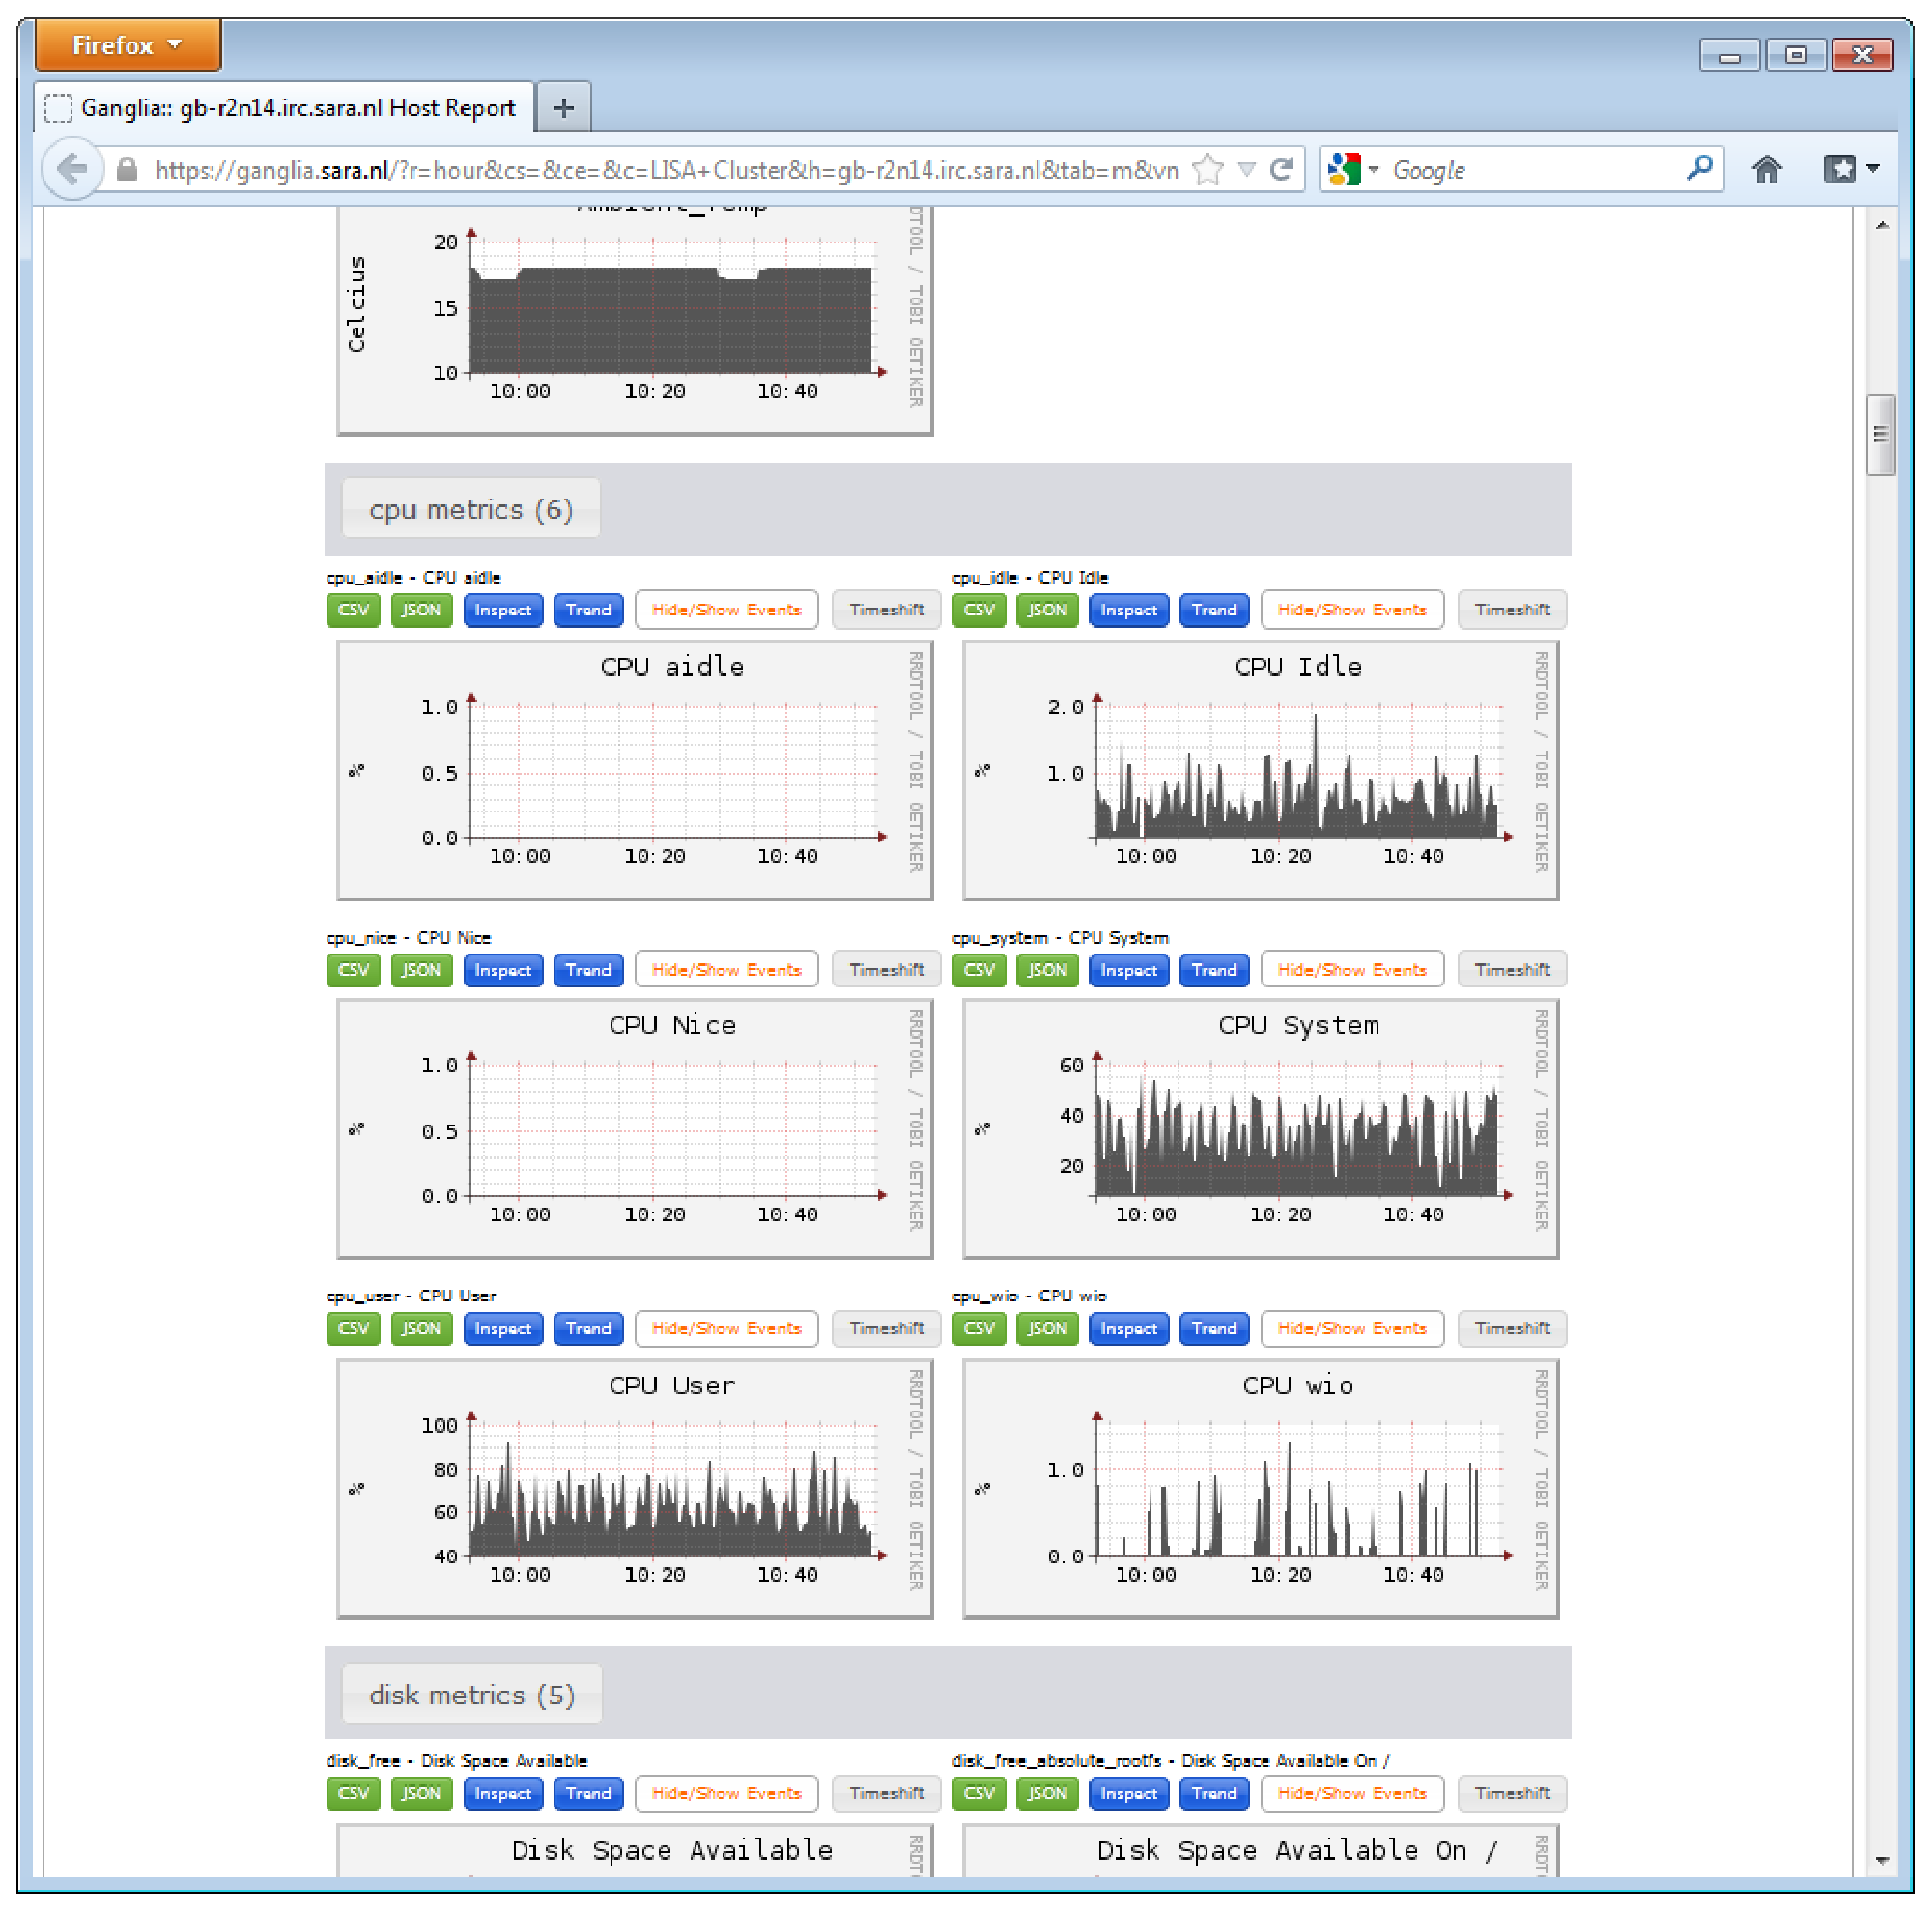
\includegraphics[width=0.9\textwidth]{./../eps/ganglia-screenshot.eps}
  \caption{Ganglia visualizes a wide array of performance indices for the LISA system. The plots can be viewed in a web browser such as Firefox.}
  \label{fig:ganglia-screenshot}
\end{figure}


Your job ends up in the express queue if it asks for less than 15~minutes walltime and doesn't use more than one node. If the system is not too busy, jobs in the express queue are usually executed without delay. In contrast, jobs that are in the batch queue can take a long time to start, but when they finally do, you can unleash the full computing power of the cluster. The interactive queue is primarily meant for development work that requires multiple machines. Submitting your job to the interactive queue is accomplished by the \lstinline[style=bashinline]{-I} option:
\begin{lstlisting}[style=basic,style=bash]
jspaaks@login4:~/tutorial$ qsub -I -lnodes=2:cores8:ppn=1 -lwalltime=00:03:00
qsub: waiting for job 6388157.batch1.irc.sara.nl to start
\end{lstlisting}
The above command asks for an interactive session with 2 nodes of the core8 type, each of which will only be running 1 process. Note that the information that is normally passed to \lstinline[style=bashinline]{qsub} through the first few lines in a jobscript (i.e.~the lines that start with \#PBS) must now be entered as options. After a delay, you will get a prompt on a different machine, in this case `gb-r7n32':

\begin{lstlisting}[style=basic,style=bash]
qsub: job 6388157.batch1.irc.sara.nl ready

jspaaks@gb-r7n32:~$ 
\end{lstlisting}
At this prompt, you can manually enter your commands, just like you were doing earlier, except you're no longer on `login4' anymore, but on one of the computing nodes within the cluster. When your time is up, the following message will appear:
\begin{lstlisting}[style=basic,style=bash]
jspaaks@gb-r7n32:~$ echo $PBS_O=>> PBS: job killed: walltime 215 exceeded limit 180
\end{lstlisting}
and you will return to `login4' (or `login3' if that's where you were before).

The \lstinline[style=bashinline]{showq} command lets you view (your part of) the queue, for example:\index{Linux commands!showq@\texttt{showq}}
\begin{lstlisting}[style=basic,style=bash]
jspaaks@login4:~/tutorial/simple-batch$ showq -u jspaaks
ACTIVE JOBS--------------------
JOBNAME            USERNAME      STATE  PROC   REMAINING            STARTTIME

6388079             jspaaks    Running     8    00:01:00  Thu Aug 23 15:41:24

     1 Active Job     6444 of 6684 Processors Active (96.41%)
                       617 of  647 Nodes Active      (95.36%)

IDLE JOBS----------------------
JOBNAME            USERNAME      STATE  PROC     WCLIMIT            QUEUETIME


0 Idle Jobs

BLOCKED JOBS----------------
JOBNAME            USERNAME      STATE  PROC     WCLIMIT            QUEUETIME


Total Jobs: 1   Active Jobs: 1   Idle Jobs: 0   Blocked Jobs: 0
jspaaks@login4:~/tutorial/simple-batch$ 
\end{lstlisting}
Also, \lstinline[style=bashinline]{showq} shows whether the cluster is very busy or not (Friday afternoons are usually the busiest, Mondays and Tuesdays are quiet in comparison). The statistics displayed by \lstinline[style=bashinline]{qsub} are updated every 15~seconds or so.


Some other commands that come in handy from time to time are:
\begin{lstlisting}[style=basic,style=bash]
jspaaks@login4:~/tutorial/simple-batch$ qdel 6388079
\end{lstlisting}\index{Linux commands!qdel@\texttt{qdel}}
This deletes job \lstinline[style=bashinline]{6388079} from the queue. Very useful if you accidentally requested too many nodes, or if your job crashed after like one second because you made a mistake. It's not possible to delete a job that was not submitted by you, so you don't have to worry about accidentally deleting other people's jobs if you type the job id wrong.

\vspace{1em}

\lstinline[style=bashinline]{checkjob} gives a more detailed overview of the job:\index{Linux commands!checkjob@\texttt{checkjob}}
\begin{lstlisting}[style=basic,style=bash]
jspaaks@login4:~/tutorial/simple-batch$ checkjob 6388672


checking job 6388672

State: Running
Creds:  user:jspaaks  group:lisa_uva  class:express  qos:DEFAULT
WallTime: 00:00:00 of 00:01:00
SubmitTime: Thu Aug 23 17:17:24
  (Time Queued  Total: 00:00:01  Eligible: 00:00:01)

StartTime: Thu Aug 23 17:17:25
Total Tasks: 1

Req[0]  TaskCount: 1  Partition: DEFAULT
Network: [NONE]  Memory >= 0  Disk >= 0  Swap >= 0
Opsys: [NONE]  Arch: x86_64  Features: [q_express][cores8]
Allocated Nodes:
[gb-r7n32:1]


IWD: [NONE]  Executable:  [NONE]
Bypass: 0  StartCount: 1
PartitionMask: [ALL]
Flags:       BACKFILL RESTARTABLE

Reservation '6388672' (00:00:00 -> 00:01:00  Duration: 00:01:00)
PE:  1.00  StartPriority:  -8641

jspaaks@login4:~/tutorial/simple-batch$ 
\end{lstlisting}

Finding out when your job is scheduled to start goes like this (the estimate is quite inaccurate in my experience):
\begin{lstlisting}[style=basic,style=bash]
showstart 6388079
\end{lstlisting}
\index{Linux commands!showstart@\texttt{showstart}}

\vspace{1em}


